\documentclass[a4paper]{article}
\usepackage[T1]{fontenc}
\usepackage[utf8]{inputenc}
\usepackage{natbib}
\usepackage{listings}
\usepackage{hyperref}
\usepackage{graphicx}

\begin{document}

\title {Modelling Rational Agents with a Genetic Algorithm}
\author{Matthia Sabatelli}

\pagestyle{empty}
\maketitle


\thispagestyle{empty}
\begin{abstract}

In the following sections we propose a computational simulation which aims to model the behaviour of some of the agents that could make use of the \textit{spyGEM} system. The model combines knowledge of different research areas such as Epistemic Logic, Machine Learning and Multi-Agent Systems. Two agents have been modelled, a possible Sender and a relative Criminal. The goal of the first one is to encrypt and send a top-secret message as safely as possible, while the criminal's goal is to avoid this possible scenario. The agents have been modelled according to the \textit{BDI Architecture}, a formal model that defines how rational agents act and behave, which has been modified and expanded specifically for this simulation. The individual parameters of this architecture have been estimated through the use of a genetic algorithm, this has been done in order to understand which parts of the architecture turn out to be more significant in a possible \textit{spyGEM} scenario.        

\end{abstract}

\section{Introduction}

Once the \textit{spyGEM} project started, before switching our attention to a broader perspective involving big data storage, we considered our idea as a possible way of sending sensitive information in a very secure way. Thanks to the combination of the Advanced Encryption Standard algorithm and the biological security layers that make it hard to get to the point in which it is possible to sequence the DNA of a bacteria, \textit{spyGEM} originally would have been the newest method to use while sending highly reserved information. Most of the research that has been done in the lab in order to make our system as safe as possible has been inspired by imagining possible scenarios involving the potential users of \textit{spyGEM}. What would happen if the agents wouldn't have enough knowledge to successfully make \textit{spyGEM} work, or what could happen if one agent would be in possession of enough sensitive information in order to make the whole procedure fail?        

Mention that we shifted from simple communication medium to bigger data storage

\section{Architecture of the Model}

The Agents have been modelled according to the \textit{BDI Architecture}, an epistemic logic based system proposed in *ref* in 1991. The paper states how important Beliefs, Desires and Intentions are in determining the behaviour of rational agents, more in detail the authors assert how every rational action taken from an agent is basically based on these three components. The combination of these features have an impact on the agent's future, in fact they have the ability to produce different actions and as a consequence give rise to different future scenarios. These possible scenarios, called \textit{Worlds}, are modelled according to a temporal structure and are defined as \textit{Time Trees}, every moment in the time tree is the result of an action based on the three previously mentioned BDI features and is defined as \textit{Situation}. One Agent can move between different time situations until it achieves its goal. The three BDI components have a different impact on the agent's behaviour and are defined as follows: 

\begin{itemize}

\item Beliefs: are defined as those worlds that the agent believes to be possible, technically every \textit{Belief} is considered as a complete and independent \textit{Time Tree} since there are no restrictions that can avoid an Agent to believe something. This feature is formalized as follows: $\forall$ w $\in$ W. \\
Where w corresponds to a single time tree and W as the entire set of beliefs. 
\item Desires: are those worlds that correspond to the optimal future scenario an agent wants to achieve, an agent can be happy with multiple outcomes but usually the main \textit{Desire} is a single one and can be expressed by the following formalism: $\exists!$ w $\in$ W 
\item Intentions: are considered as sets of intention-accessible worlds. These worlds are ones that the agent has committed to attempt to realize. Differently from the \textit{Beliefs}, where all possible worlds are considered, the \textit{Intention} feature is characterized by a strong component of realism since the worlds that are part of this feature are only the ones that the Agent thinks can be a possible \textit{Desire}. Intentions are formalized as follows:

\end{itemize} 

In addition to the three BDI features some extra parameters have been added in order to model the agents. The reason this has been done is related to the genetic algorithm that has been used in order to simulate their behaviour and is explained into more detail in the next section. The parameters that have been added to the architecture are different according to the type of agent that has been modelled, however the general idea is the same one for both of them. In order to represent a potential level of \textit{Beliefs, Desires} and \textit{Intentions} in a \textit{spyGEM} scenario some extra features related to this specific world have been added that might have an impact on all three BDI components and as a consequence on the agents' actions. \\
Regarding a potential \textit{Sender} the three additional features that have been added are the following:
\begin{itemize}
\item $\gamma$: which corresponds to a particular level of \textit{riskiness} the agent will take into account in his actions. The impact of this feature is different on the three BDI components, in fact a high level of riskiness makes the agent have a smaller set of total \textit{Beliefs} since there is no reason to think about all those worlds that involve highly safe scenarios. On the other side it is possible that a high level of $\gamma$ leads to the optimal desired world and as a consequence to a world the agent thinks requires commitment.  
\item $\psi$: is a variable that is related to the level of \textit{efficiency} that the agent wants to pursue in its actions. In this case the higher this value is the higher the value of the three BDI components will be. 
\item $\alpha$: corresponds to the \textit{time resources} the agent is willing to invest when creating its BDI features, the impact of this variable is similar to the previous one. The more time that is invested by an agent, the higher the set of Beliefs will be and the overall commitment to the possible worlds towards the optimal scenario.
\end{itemize}

Regarding the \textit{Criminal} Agent the meaning of $\psi$ and $\alpha$ has been changed. The first value corresponds to the amount of knowledge the agent has about the different \textit{Time Trees} while the second one is related to the amount of motivation and effort he is willing to put while interfering with the \textit{Sender's} plan. \\
    
The idea of the model was to identify which of the three BDI components is considered as more important by a potential \textit{Sender} agent who wants to hide and send an encrypted message as safely as possible and by a \textit{Criminal} who wants to avoid this scenario. In order to find this out a genetic algorithm has been used on different randomly generated agents and the level of the three BDI features has been measured once the algorithm converged to the optimal result. \\
Genetic algorithms are a very common machine learning technique that is used in different Artificial Intelligence optimization problems, they are largely inspired by natural evolution and work as follows: a random set of possible solutions is created, each of these solutions goes through a fitness function which measures how close these solutions perform to the optimal result that wants to be achieved. It is important to notice that the individual values that make it possible to converge to the optimal result are not known beforehand, the only information that is known is the final outcome which can be achieved in multiple ways.\\
Once the agents are evaluated by the fitness function a truncation process occurs, similarly as what happens in nature where only the fittest animals survive, also in the simulation the only agents that are allowed to be part and give rise to a new generation are the ones with higher fitness scores. How new generations are created more into detail is presented in the next subsection.


\subsection{The Sender}

An Agent is created as a string of binary bits and is represented as a chromosome, each part of it represents the three BDI features together with the three additional parameters mentioned in the previous section. An example of a randomly generated agent is the following:

\begin{equation}
	Chromosome_1 = \underbrace{010010011010}_{Beliefs}\underbrace{011101110101}_{Intentions}\underbrace{010100101010}_{Desires}
\end{equation}

\begin{equation}
	Beliefs = \underbrace{0100}_{\gamma} \underbrace{1001}_{\psi} \underbrace{1010}_{\alpha} 
\end{equation}  

Every binary pair corresponds to a decimal number that if converted properly and summed together establishes the total fitness value of the chromosome. For the sender Agent an optimal value of 60 has been set, this turned out in the following fitness function, where n is the total length of the chromosome and the main aim is to find the optimal set of bits that satisfy it:

\begin{equation}
	f(x) = \sum\limits_{i=0}^{n} x[i] = 60
\end{equation} 

For our \textit{Sender} simulation the following parameters turned out to be the most suitable ones while considering optimal convergence performance and training time:

\begin{itemize}

\item 20 Simulations: a total number of twenty different simulations have been run in order to check if the results where coherent between each other.
\item 20 Pools of 100 Chromosomes: the simulation starts with 20 randomly generated chromosome pools with 100 agents each. This is the first set of agents that is evaluated by the fitness function and according to the fitness scores the breeding process starts. 
\item Truncation Method: is the approach that has been used in order to keep the fittest agents allowed to reproduce themselves, in order to avoid overfitting issues the top 70\% of the agents has been kept while the rest 30\% has been discarded.
\item One point single crossover: is the breeding method that has been used. Once two chromosomes are chosen as parents they give birth to two new children by exchanging 3 of their bits. This technique is shown hereafter:

\begin{equation}
	Parent_1 = \underbrace{\textbf{010}}_{Crossover Bits}{010011010011101110101010100101010}
\end{equation}
\begin{equation}
	Parent_2 = \underbrace{\textbf{011}}_{Crossover Bits}{010000010011101111001010111101000}
\end{equation}
\begin{equation}
	Child_1 = \underbrace{010}_{Parent 1 Bits} \underbrace{010000010011101111001010111101000}_{Parent 2 Bits}
\end{equation}
\begin{equation}
	Child_2 = \underbrace{011}_{Parent 2 Bits}\underbrace{010011010011101110101010100101010}_{Parent 2 Bits}
\end{equation}

\item 1\% mutation rate: some randomness has to be added to the newest generation in order to make the pool more varied and avoid local minima, in our case a 1\% mutation rate has been set which means that one bit of one chromosome is randomly changed from 0 to 1 or vice-versa.  

\end{itemize}

The following two figures show the results of the genetic algorithm and the analysis of the three different BDI features.

\begin{figure}[ht!]
\minipage{0.45\textwidth}
   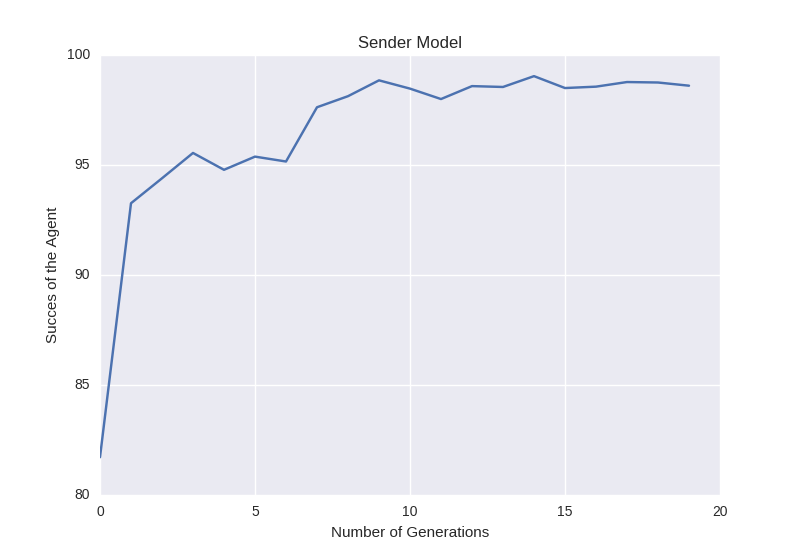
\includegraphics[width=\linewidth]{goodCOnv_7.png}
  \caption{The graph shows how after 20 generations of breeding the pool of chromosomes representing the \textit{Sender} agents converge to the optimal result. Generation 4 and 11 show some local minima that thanks to the random mutation present in the genetic algorithm don't impede the achievement of the optimal convergence.}\label{fig:awesome_image1}
\endminipage\hfill
\minipage{0.45 \textwidth}
  \includegraphics[width=\linewidth]{SenderBDI.png}
  \caption{Histogram with the analysis of the BDI features. On the \textit{x-axis} the decimal value represting that feature is presented while on the \textit{y-axis} its amount of occurances during the simulation. The different colors in the historgram represent the different BDI components: Beliefs are shown in yellow, Desires in blue and Intentions in red. The results show how the Belief feature is the one that the Agents discard in order to get to the optimal score, in fact for 15 times it is the BDI component with the lowest value, 6. This is remarkable since it shows how not too many resources should be invested in imagining all possible scenarios but it is better to have a strong set of Desires that nicely match with the Intention to pursue one of those. This is shown in the graph where an optimal value of 13 has been chosen by the Agents regarding these two BDI components for more then 20 times.}\label{fig:awesome_image2}
\endminipage\hfill
\end{figure}


\subsection{The Criminal}

\section{Discussion and Conclusion}


\section{References}

Rao, A. S., \& George, M. P. (1991). Modeling Rational Agents within a BDI-Architecture. \\

Herrera, F., \& Verdegay, J. L. (1996). Genetic algorithms and soft computing. Physica-Verlag. \\

Zhong, W., Liu, J., Xue, M., \& Jiao, L. (2004). A multiagent genetic algorithm for global numerical optimization. IEEE Transactions on Systems, Man, and Cybernetics, Part B (Cybernetics), 34(2), 1128-1141. \\

Goldberg, D. E., \& Holland, J. H. (1988). Genetic algorithms and machine learning. Machine learning, 3(2), 95-99. \\

It is possible to download the software that models the agents with the genetic algorithm from here: \url{https://github.com/paintception/myGEM}


\end{document}
